\section*{Materiais e Métodos}

%%%%%%%%%%%%%%%%%%%%%%%%%%%%%%%%%%%%%%%%%%%
%% VISÃO GERAL
%%%%%%%%%%%%%%%%%%%%%%%%%%%%%%%%%%%%%%%%%%%
\subsection*{Visão Geral}

\begin{figure}[h!]
  \centering
  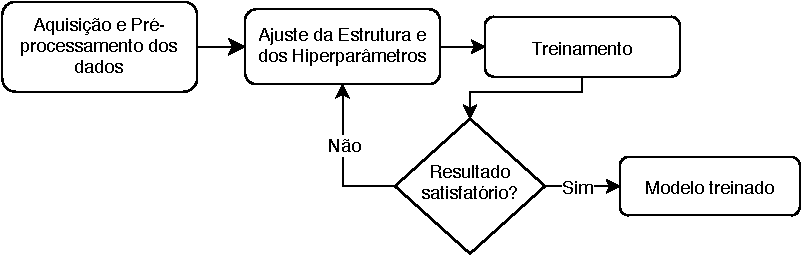
\includegraphics[width=\textwidth]{figures/dl_diagram.pdf}
  \caption{Fluxograma do desenvolvimento do modelo.}
  \label{fig:fluxogram}
\end{figure}

Pelo fluxograma da figura \ref{fig:fluxogram}, vemos que a primeira etapa no desenvolvimento da Rede Neural Convolucional é a aquisição e o pré-processamento dos dados. A criação da estrutura (sequência de camadas da rede neural) e o ajuste dos hiperparâmetros, também chamdo de \emph{fine tunning}, vem em seguida. É o treimento que une a primeira e a segunda etapa, pois é nele que os dados pré-processados são inseridos na estrutura modelada. Logo em seguida, é feita uma validação da rede treinada. É o desempenho da modelagem anterior que dá o \emph{feedback} das modificações necessárias para a próxima versão da estrutura. O desenvolvimento do modelo termina quando é atingida uma boa acurácia de predição.

%%%%%%%%%%%%%%%%%%%%%%%%%%%%%%%%%%%%%%%%%%%%%
%% AQUISIÇÃO DOS DADOS
%%%%%%%%%%%%%%%%%%%%%%%%%%%%%%%%%%%%%%%%%%%%%
\subsection*{Aquisição dos dados}

Dados de treinamento são elementos fundamentais para o treinamento supervisionado de uma Rede Neural Artificial. Para treinar uma rede que aprenda a classificar galáxias de acordo com suas imagens é necessário fazê-la aprender formas e padrões das galáxias. Para isso, é necessário separar uma grande amostra de imagens de galáxias já classificadas por humanos.

A fonte dos dados são GalaxyZoo, que contém as classificações morfológicas, e SDSS, que possui as imagens das galáxias. A associação dos dados entre estas duas fontes são feitas pelas coordenadas do objeto no espaço.

\begin{figure}[h!]
  \centering
  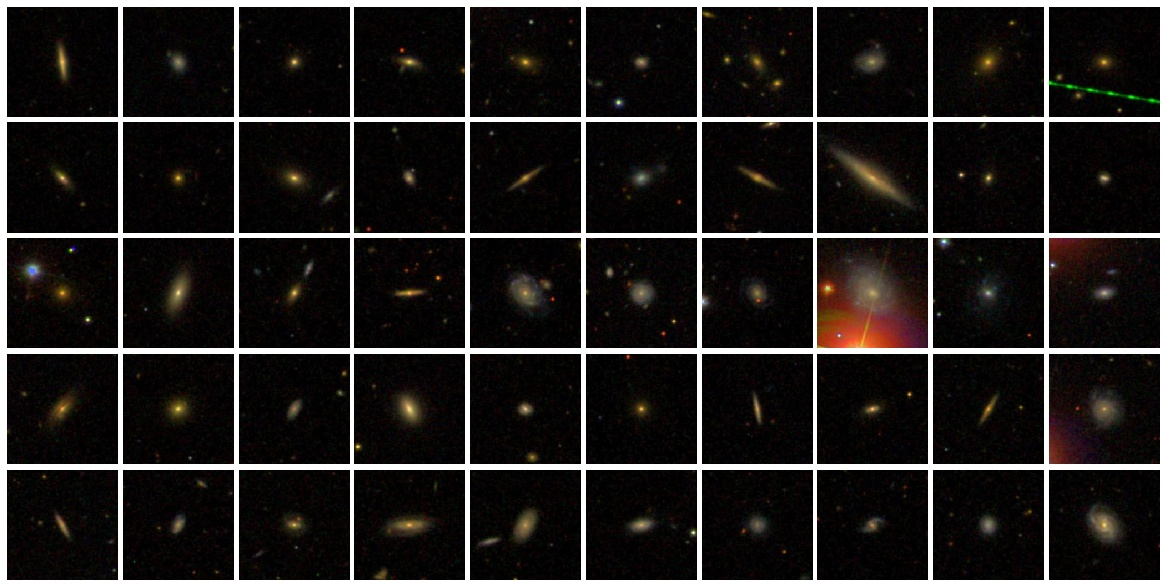
\includegraphics[width=\textwidth]{figures/galaxy_grid.jpg}
  \caption{Amostra com cinquenta imagens de galáxias (escala reduzida).}
  \label{fig:galaxy_grid}
\end{figure}

O catálogo com as classificações estão em um arquivo CSV. Já as imagens foram obtidas usando a \emph{API}\footnote{API: \emph{Application Programming Interface}. É uma interface de comicação entre sistemas.} do SDSS\footnote{Documentação da API: http://skyserver.sdss.org/dr16/en/help/docs/api.aspx.}. Para acessar a imagem de uma galáxia, o \emph{endpoint}\footnote{O endpoint é o ponto final de um canal de comunicação, ou seja, é a URL acessada para executar alguma função no servidor.} da API do SDSS requer pelo menos dois parâmetros: a ascensão reta\footnote{Distância angular de um ponto específico medido para o leste ao longo do equador celeste.} (RA) e a declinação\footnote{Ângulo que localiza um ponto na esfera celeste no sistema de coordenadas equatoriais.} (DEC).

O algorítmo\cite{cardoso2020} baixa todas as imagens de galáxias que estão no catálogo do GalaxyZoo usando a API do SDSS. A figura \ref{fig:galaxy_grid} contém uma amostra de cinquenta imagens de galáxias obtidas pelo algorítmo.

Foram baixadas 108.286 imagens no formato JPG e modelo de cores RGB, cada uma com dimensão de 200x200 pixels e escala de 1,35 arsec/pixel do objeto.

%%%%%%%%%%%%%%%%%%%%%%%%%%%%%%%%%%%%%%%%%%%%%%
%% PRÉ-PRECESSAMENTO DOS DADOS
%%%%%%%%%%%%%%%%%%%%%%%%%%%%%%%%%%%%%%%%%%%%%%
\subsection*{Pré-processamento dos dados}

O pré-processamento é a preparação das imagens para serem usadas pelo modelo durante o treinameto. As imagens são separadas em cinco classes: \texttt{Ei}, \texttt{Er}, \texttt{Ec}, \texttt{Ser}, \texttt{Sc2m} e foram agrupadas em três subconjuntos: treinamento, validação e teste.

\begin{table}[h!]
  \centering
  \renewcommand{\arraystretch}{1.6}
  \begin{tabular}{ccccc}
    \toprule
    \thead{Classe} & \thead{Treinamento\\(82,5\%)} & \thead{Validação\\(15\%)} & \thead{Teste\\(2,5\%)} & \thead{Total} \\ 
    \midrule
    Ei      & 36.333    & 6.605     & 1.100     & 44.038 \\
    Er      & 30.331    & 5.514     & 919       & 36.764 \\
    Ser     & 11.558    & 2.101     & 350       & 14.009 \\
    Ec      & 8.374     & 1.522     & 253       & 10.149 \\
    Sc2m    & 2.745     & 498       & 83        & 3.326 \\ 
    Total   & 89.341    & 16.240    & 2.705     & 108.286 \\
    \bottomrule
  \end{tabular}
  \caption{Quantidade de amostras de imagens de galáxias por classe.}
  \label{tab:img_qtd}
\end{table}

Para cada subconjunto é separada uma quantidade de amostras relativa à quantidade total de cada classe: sendo 82,5\% para o treino, 15\% para a validação e 2,5\% para o teste. A tabela \ref{tab:img_qtd} mostra a quantidade de imagens para cada um dos subconjuntos conforme a classe.

Depois de separadas, as imagens precisam ser transformadas em tensores. No sistema RGB, cada cor é representada por três números inteiros no intervalo de 0 a 255. Cada imagem, então, é representada por um tensor de dimensão (200, 200, 3). As primeiras duas dimensões são referentes ao comprimento e largura da imagem e a terceira aos três canais de cores RGB.

Representar uma cor por um terno faz sentido quando se conhece a especificação do sistema de cores RGB, mas isso não é intuituvo para um modelo de rede neural artificial. Por isso, cada número do tensor é reescalado para um número real no intervalo entre zero e um dividindo cada número por 255.

%%%%%%%%%%%%%%%%%%%%%%%%%%%%%%%%%%%%%%%%%%%%%%
%% MODELAGEM DA REDE NEURAL ARTIFICIAL
%%%%%%%%%%%%%%%%%%%%%%%%%%%%%%%%%%%%%%%%%%%%%%
\subsection*{Modelagem e Ajuste dos Hiperparâmetros}

A rede neural artificial foi programada em Python e a biblioteca Keras\footnote{Uma API de alto nível criada para modelagem e treinamento de redes neurais que, neste projeto, roda sobre o TensorFlow. Tem foco em permitir experimentação rápida.} foi usada para criar e treinar o modelo.

A modelagem é a criação de uma estrutura. Isto inclui: a escolha da quantidade de camadas, a definição do tipo de cada camada e a especificação da sequência em que as camadas aparecerão. Já os hiperparâmetros são os atributos de cada camada ou do modelo em geral. Alguns exemplos de hiperparâmetros são: a taxa de aprendizagem\footnote{A velocidade com que a rede neural aprende os padrões.} (\emph{learning rate}), a quantidade de unidades\footnote{A quantidade de neurônios artificais.} de cada camada e a taxa (\emph{rate}) das camadas \emph{dropout}. Estes ajustes são feitos empiricamente e reajustados de acordo com o resultado obtido após o treinamento, como visto na figura \ref{fig:fluxogram}.

\pagebreak

\begin{figure}[h!]
  \centering
  \begin{minipage}[t]{.47\textwidth}
    \centering
    \tikzset{
>=stealth',
  punktchain/.style={
    rectangle, 
    rounded corners, 
    % fill=black!10,
    draw=black, thick,
    text width=8em, 
    minimum height=2em, 
    text centered, 
    on chain},
  line/.style={draw, thick, <-},
  element/.style={
    tape,
    top color=white,
    bottom color=blue!50!black!60!,
    minimum width=8em,
    draw=blue!40!black!90, very thick,
    text width=8em, 
    minimum height=2em, 
    text centered, 
    on chain},
  every join/.style={->, thick, shorten >=1pt},
}

\begin{tikzpicture}
    [node distance=.5cm,
    start chain=going below,]
    \node[punktchain, join] (input) {\small Input};
    \node[punktchain, join] (conv_1) {\small Conv2D};
    \node[punktchain, join] (maxpool_1) {\small MaxPooling2D};
    \node[punktchain, join] (conv_2) {\small Conv2D};
    \node[punktchain, join] (maxpool_2) {\small MaxPooling2D};
    \node[punktchain, join] (conv_3) {\small Conv2D};
    \node[punktchain, join] (maxpool_3) {\small MaxPooling2D};
    \node[punktchain, join] (conv_4) {\small Conv2D};
    \node[punktchain, join] (maxpool_4) {\small MaxPooling2D};
    \node[punktchain, join] (flatten) {\small Flatten};
    \node[punktchain, join] (dense_1) {\small Dense};
    \node[punktchain, join] (dense_2) {\small Dense};
\end{tikzpicture}
    \captionof{figure}{\textbf{Modelo 1} -- Camadas convolucionais intercaladas com camadas \emph{pooling}.}
    \label{fig:conv_model}
  \end{minipage}%
  \hfill%
  \begin{minipage}[t]{.47\textwidth}
    \centering
    \tikzset{
  >=stealth',
  punktchain/.style={
      rectangle,
      rounded corners,
      draw=black, thick,
      text width=8em,
      minimum height=2em,
      text centered,
      on chain},
  line/.style={draw, thick, <-},
  every join/.style={->, thick, shorten >=1pt},
}

\begin{tikzpicture}
  [node distance=.5cm,
    start chain=going below,]
  \node[punktchain, join] (input) {\small Input};
  \node[punktchain, join] (vgg16) {\small VGG16};
  \node[punktchain, join] (flatten) {\small Flatten};
  \node[punktchain, join] (dense_1) {\small Dense};
  \node[punktchain, join] (dropout_1) {\small Dropout};
  \node[punktchain, join] (dense_2) {\small Dense};
  \node[punktchain, join] (dropout_2) {\small Dropout};
  \node[punktchain, join] (dense_3) {\small Dense};
  \node[punktchain, join] (dropout_3) {\small Dropout};
  % \node[punktchain, join] (dense_4) {\small Dense};
  % \node[punktchain, join] (dropout_4) {\small Dropout};
  \node[punktchain, join] (dense_5) {\small Dense};
\end{tikzpicture}
    \captionof{figure}{\textbf{Modelo 2} -- Rede pré-treinada ligada à uma rede densa com \emph{dropout}.}
    \label{fig:pretrained_model}
  \end{minipage}
  \end{figure}

\pagebreak

Foram criados dois modelos: um, usando apenas camadas convolucionais e \emph{pooling} ligadas a uma pequena rede densa (figura \ref{fig:conv_model}) e outro, usando uma rede pré-treinada, VGG16, ligada a uma longa rede densa com \emph{dropout} de acordo com o diagrama da figura \ref{fig:pretrained_model}.

Cada modelo representa uma técnica diferente para treinamento de redes neurais. A primeira, que é a mais \emph{canônica}, usa apenas informações do conjunto de treinamento, já a segunda usa pesos definidos de uma rede neural pré-treinada, VGG16. 

Esta rede VGG16 é treinada usando a base de dados \emph{ImageNet}\footnote{http://www.image-net.org/.}, que possui milhões de imagens de objetos do cotidaino, mas não possui objetos do espaço. A idéia é descobrir que se usar uma rede pré-treinada com milhões de imagens, mas nenhuma de galáxias, é tão relevante quanto usar uma rede treinada com apenas alguns milhares de amostras, mas todas de galáxias. Pois as redes neurais convolucionais são usadas como camada de abstração do mundo visual, ou seja, elas detectam padrões como geometrias, texturas e cores.

Para ambos os modelos, a dimensão do tensor da entrada é (200, 200, 3). Cinco unidades na camada de saída com ativador \texttt{Softmax}. A  função de perda utilizada foi a \texttt{Categorical Crossentropy} e o otimizador foi o \texttt{RMSprop}.

\begin{table}[h!]
  \centering
  \begin{tabular}{cc}
    \toprule
    \thead{Hiperparâmetro} & \thead{Valor} \\
    \midrule
    Ativador (Conv2D) & ReLu \\
    Ativador (Dense, 1) & ReLu \\
    Unidades (Conv2D) & 32, 64, 128 e 128 \\
    Unidades (Dense, 1) & 512 \\
    Dimensão do Kernel (Conv2D) & (3, 3) \\
    \emph{Pool Size} (MaxPooling2D) & (2, 2) \\
    Taxa de aprendizagem & $10^{-4}$ \\
    \bottomrule
  \end{tabular}
  \caption{Descrição dos hiperparâmetros do Modelo 1.}
  \label{tab:hip_model1}
\end{table}

\begin{table}[h!]
  \centering
  \begin{tabular}{cc}
    \toprule
    \thead{Hiperparâmetro} & \thead{Valor} \\
    \midrule
    Ativador (Dense, 1-4) & ReLu \\
    Unidades (Dense, 1-4) & 2048, 1024, 512, 256 \\
    Taxa de \emph{dropout} & 0,5 \\
    Taxa de aprendizagem & $10^{-5}$ \\
    \bottomrule
  \end{tabular}
  \caption{Descrição dos hiperparâmetros do Modelo 2.}
  \label{tab:hip_model2}
\end{table}

Como mostrado na figura \ref{fig:fluxogram}, diversos valores de hiperparâmetros foram ajustados empiricamente. As tabelas \ref{tab:hip_model1} e \ref{tab:hip_model2} mostram os valores dos hiperparâmetros com melhor desempenho e que são usados como exemplo nos resultados.